\documentclass{beamer}

\usepackage{amsmath, tikz, subfigure, graphicx}
\usetikzlibrary{decorations.pathreplacing,decorations.pathmorphing,arrows,positioning,shapes,shapes.multipart}

\title[FTFP]{Approximation Algorithms
  for the Fault-Tolerant Facility Placement Problem}
\author[lyan]{Li Yan}
\institute[UCR]{
  Computer Science\\
  University of California Riverside\\
}
\date{06/10/2013}
\usetheme{Warsaw}


%%%%%%%%%%%%%%%%%%%%%%%%%%%%%%%%%%%%%%%%%%%%%%%%%%%%%%%%%%

% non-math stuff

\newcommand{\myparagraph}[1]{{\medskip\noindent{\bf #1}}}
\newcommand{\emparagraph}[1]{{\medskip\noindent{\it #1}}}
\newcommand{\etal}{{\it et al.}}
\newcommand{\myif}{{\mbox{\rm\ if \ }}}
\newcommand{\mycase}[1]{\mbox{{\underline{Case #1}}:\/}}

\newcommand{\margincomment}[1]%
    {{%
      \marginpar{{\tiny\begin{minipage}{0.5in}
                       \begin{flushleft}
                          {#1}
                       \end{flushleft}
                       \end{minipage}
                }}
    }}


%%%%%%%%%%%%%%%%%%%%%%%%%%%%%%%%%%%%%%%%%%%%%%%%%%%%%%%%%%

% various letters

\newcommand{\hatc}{{\hat c}}
\newcommand{\hatC}{{\hat C}}
\newcommand{\hatr}{{\hat r}}
\newcommand{\hatx}{{\hat x}}
\newcommand{\haty}{{\hat y}}
\newcommand{\dotx}{{\dot x}}
\newcommand{\doty}{{\dot y}}
\newcommand{\dotr}{{\dot r}}
\newcommand{\boldx}{{\mathbf x}}

\newcommand{\doubledone}{{\bar 1}}
\newcommand{\doubledtwo}{{\bar 2}}
\newcommand{\barc}{{\bar c}}
\newcommand{\bart}{{\bar t}}

\newcommand{\barx}{{\bar x}}
\newcommand{\bary}{{\bar y}}
\newcommand{\barz}{{\bar z}}
\newcommand{\barr}{{\bar r}}
\newcommand{\barX}{{\bar X}}
\newcommand{\barY}{{\bar Y}}
\newcommand{\barZ}{{\bar Z}}
\newcommand{\bara}{{\bar a}}
\newcommand{\bard}{{\bar d}}
\newcommand{\barm}{{\bar m}}
\newcommand{\barA}{{\bar A}}
\newcommand{\barB}{{\bar B}}
\newcommand{\barC}{{\bar C}}
\newcommand{\barG}{{\bar G}}
\newcommand{\barE}{{\bar E}}
\newcommand{\barV}{{\bar V}}

\newcommand{\wbarC}{{\overline{C}}}
\newcommand{\wbarD}{{\overline{D}}}
\newcommand{\wbarN}{{\overline{N}}}
\newcommand{\wbarX}{{\overline{X}}}


\newcommand{\barbeta}{{\bar\beta}}
\newcommand{\bargamma}{{\bar\gamma}}
\newcommand{\apomega}{{\bar\omega}}

\newcommand{\bfr}{\boldsymbol{r}}
\newcommand{\bfv}{{\bf v}}
\newcommand{\bfx}{\boldsymbol{x}}
\newcommand{\bfy}{\boldsymbol{y}}
\newcommand{\bfz}{{\bf z}}
\newcommand{\bfQ}{{\bf Q}}
\newcommand{\bfR}{{\bf R}}
\newcommand{\bfS}{{\bf S}}
\newcommand{\bfT}{{\bf T}}
\newcommand{\bfV}{{\bf V}}
\newcommand{\bfone}{{\bf 1}}
\newcommand{\bfalpha}{\boldsymbol{\alpha}}
\newcommand{\bfbeta}{\boldsymbol{\beta}}

\newcommand{\calA}{{\cal A}}
\newcommand{\calB}{{\cal B}}
\newcommand{\calC}{{\cal C}}
\newcommand{\calD}{{\cal D}}
\newcommand{\calE}{{\cal E}}
\newcommand{\calG}{{\cal G}}
\newcommand{\calH}{{\cal H}}
\newcommand{\calJ}{{\cal J}}
\newcommand{\calK}{{\cal K}}
\newcommand{\calL}{{\cal L}}
\newcommand{\calM}{{\cal M}}
\newcommand{\calN}{{\cal N}}
\newcommand{\calS}{{\cal S}}
\newcommand{\calU}{{\cal U}}
\newcommand{\calX}{{\cal X}}
\newcommand{\calT}{{\cal T}}

\newcommand{\hatcalI}{{\hat{\cal I}}}
\newcommand{\barcalI}{{\bar{\cal I}}}
\newcommand{\dotcalI}{{\dot{\cal I}}}

\newcommand{\vecS}{{\bar S}}
\newcommand{\vecT}{{\bar T}}
\newcommand{\vecone}{{\bf 1}}
\newcommand{\tildec}{{\tilde c}}
\newcommand{\tilded}{{\tilde d}}
\newcommand{\tildeD}{{\tilde D}}
\newcommand{\tildeC}{{\widetilde C}}
\newcommand{\tildeZ}{{\tilde Z}}
\newcommand{\tilder}{{\widetilde r}}
\newcommand{\tildex}{{\widetilde x}}
\newcommand{\wtildeN}{{\widetilde N}}
\newcommand{\tildebfr}{\widetilde{\boldsymbol{r}}}
\newcommand{\tildebfx}{\widetilde{\boldsymbol{x}}}
\newcommand{\tildebfy}{\widetilde{\boldsymbol{y}}}

\newcommand{\barbfx}{\bar{\boldsymbol{x}}}
\newcommand{\barbfy}{\bar{\boldsymbol{y}}}
\newcommand{\hatbfx}{\hat{\boldsymbol{x}}}
\newcommand{\hatbfy}{\hat{\boldsymbol{y}}}
\newcommand{\dotbfx}{\dot{\boldsymbol{x}}}
\newcommand{\dotbfy}{\dot{\boldsymbol{y}}}

\newcommand{\wbarcalC}{{\overline{\calC}}}
\newcommand{\wbarcalD}{{\overline{\calD}}}
\newcommand{\eps}{{\epsilon}}

%%%%%%%%%%%%%%%%%%%%%%%%%%%%%%%%%%%%%%%%%%%%%%%%%%%%%%%%%%

\newcommand{\half}{{\mbox{$\frac{1}{2}$}}}
\newcommand{\threehalfs}{{\mbox{$\frac{3}{2}$}}}
\newcommand{\threefourths}{{\mbox{$\frac{3}{4}$}}}
\newcommand{\fivehalfs}{{\mbox{$\frac{5}{2}$}}}
\newcommand{\onethird}{{\mbox{$\frac{1}{3}$}}}
\newcommand{\twothirds}{{\mbox{$\frac{2}{3}$}}}
\newcommand{\fourthirds}{{\mbox{$\frac{4}{3}$}}}
\newcommand{\fivethirds}{{\mbox{$\frac{5}{3}$}}}
\newcommand{\fivefourths}{{\mbox{$\frac{5}{4}$}}}
\newcommand{\onefourth}{{\mbox{$\frac{1}{4}$}}}
\newcommand{\onefifth}{{\mbox{$\frac{1}{5}$}}}
\newcommand{\twofifths}{{\mbox{$\frac{2}{5}$}}}
\newcommand{\threefifths}{{\mbox{$\frac{3}{5}$}}}
\newcommand{\fourfifths}{{\mbox{$\frac{4}{5}$}}}
\newcommand{\ninefifths}{{\mbox{$\frac{9}{5}$}}}
\newcommand{\sevensixths}{{\mbox{$\frac{7}{6}$}}}
\newcommand{\oneeighth}{{\mbox{$\frac{1}{8}$}}}
\newcommand{\threeeighths}{{\mbox{$\frac{3}{8}$}}}
\newcommand{\fiveeighths}{{\mbox{$\frac{5}{8}$}}}
\newcommand{\seveneighths}{{\mbox{$\frac{7}{8}$}}}
\newcommand{\onetenth}{{\mbox{$\frac{1}{10}$}}}
\newcommand{\seventenths}{{\mbox{$\frac{7}{10}$}}}
\newcommand{\ninetenths}{{\mbox{$\frac{9}{10}$}}}
\newcommand{\twonineths}{{\mbox{$\frac{2}{9}$}}}
\newcommand{\fivenineths}{{\mbox{$\frac{5}{9}$}}}
\newcommand{\elevennineths}{{\mbox{$\frac{11}{9}$}}}
\newcommand{\threetwentieths}{{\mbox{$\frac{3}{20}$}}}
\newcommand{\twentyfivenineteenths}{{\mbox{$\frac{25}{19}$}}}

\newcommand{\sqrttwo}{\sqrt{2}}

%%%%%%%%%%%%%%%%%%%%%%%%%%%%%%%%%%%%%%%%%%%%%%%%%%%%%%%%%%

% various delimiters

\newcommand{\braced}[1]{{ \left\{ #1 \right\} }}
\newcommand{\angled}[1]{{ \left\langle #1 \right\rangle }}
\newcommand{\brackd}[1]{{ \left[ #1 \right] }}
\newcommand{\parend}[1]{{ \left( #1 \right) }}
\newcommand{\barred}[1]{{ \left| #1 \right| }}
\newcommand{\dbarred}[1]{{ \left\| #1 \right\| }}
\newcommand{\floor}[1]{{ \lfloor #1 \rfloor }}
\newcommand{\ceiling}[1]{{ \lceil #1 \rceil }}

%%%%%%%%%%%%%%%%%%%%%%%%%%%%%%%%%%%%%%%%%%%%%%%%%%%%%%%%%%

% some math symbols

\newcommand{\set}{\,{\leftarrow}\,}
\newcommand{\suchthat}{{\,:\,}}
\newcommand{\cost}{{\it cost}}
\newcommand{\yield}{{\it yield}}
\newcommand{\opt}{{\it opt}}

\newcommand{\algA}{{\bf A}}
\newcommand{\LHS}{{\rm LHS}}
\newcommand{\RHS}{{\rm RHS}}
\newcommand{\reals}{{\bf R}}
\newcommand{\posreals}{{\bf R}^+}

\newcommand{\assign}{{\,\leftarrow\,}}

\newcommand{\absvalue}[1]{{\barred{#1}}}
\newcommand{\posvalue}[1]{{\brackd{#1}^+}}

\newcommand{\NP}{{\mbox{\sf NP}}}
\newcommand{\PP}{{\mbox{\sf P}}}
\newcommand{\DTIME}{{\mbox{\sf DTIME}}}

\newcommand{\letbox}[1]{{\makebox[11pt]{{\small {$#1$}}}}}
\newcommand{\optstring}[1]{{ \frame{\;\raisebox{0pt}[12pt][5pt]{#1}\;} }}

\newcommand{\leftend}{{\diamond}}
\newcommand{\rightend}{{\diamond}}

%\newcommand{\argmin}{{\mbox{\rm argmin}}}
\DeclareMathOperator*{\argmin}{arg\,min}

\newcommand\litem[1]{\item{\bfseries #1\enspace}}
\newcommand{\ceil}[1] {\lceil #1 \rceil}
\newcommand{\naive}{na\"{\i}ve}
\newcommand{\LP}{\mbox{\rm LP}}
\newcommand{\OPT}{\mbox{\rm OPT}}
\newcommand{\ALG}{\mbox{\rm ALG}}
\newcommand{\LPR}[1]{{\mbox{\rm LPR#1}}}
\newcommand{\smallLPR}[1]{{\mbox{\tiny\rm LPR#1}}}
% algorithm names
\newcommand{\ESTA}{\mbox{\rm ESTA}} % 4approx
\newcommand{\EGUP}{\mbox{\rm EGUP}} % 3approx
\newcommand{\ECHS}{\mbox{\rm ECHS}} % 1.736
\newcommand{\EBGS}{\mbox{\rm EBGS}} % 1.575
\newcommand{\GUP}{\mbox{\rm GUP}}
\newcommand{\smallESTA}{\mbox{\tiny\rm ESTA}}
\newcommand{\smallEGUP}{\mbox{\tiny\rm EGUP}}
\newcommand{\smallECHS}{\mbox{\tiny\rm ECHS}}
\newcommand{\smallEBGS}{\mbox{\tiny\rm EBGS}}

\newcommand{\SOL}[1]{{{\mbox{\rm SOL}}_{#1}}}
\newcommand{\FTFP}{\mbox{\rm FTFP}}
\newcommand{\FTFL}{\mbox{\rm FTFL}}
\newcommand{\calI}{\mathcal{I}}
\newcommand{\avg}{{\mbox{\scriptsize\rm avg}}}

\newcommand{\dmax}{\text{dmax}}
\newcommand{\davg}{\text{davg}}
\newcommand{\favg}{f_{\text{avg}}}
\newcommand{\conn}{\text{conn}}
\newcommand{\cls}{\text{cls}}
\newcommand{\far}{\text{far}}

\newcommand{\sitesset}{\mathbb{F}}
\newcommand{\clientset}{\mathbb{C}}
\newcommand{\facilityset}{\overline{\sitesset}}
\newcommand{\demandset}{\overline{\clientset}}

%\newcommand{\dist}{{\mbox{dist}}}
\newcommand{\concost}{C^{\avg}}
\newcommand{\faccost}{F^{\avg}}
\newcommand{\tcc}{\mbox{\rm{tcc}}}
\newcommand{\clsdist}{C_{\cls}^{\avg}}
\newcommand{\fardist}{C_{\far}^{\avg}}
\newcommand{\clsmax}{C_{\cls}^{\max}}
\newcommand{\clsnb}{N_{\cls}}
\newcommand{\farnb}{N_{\far}}
\newcommand{\wbarclsnb}{\wbarN_{\cls}}
\newcommand{\wbarfarnb}{\wbarN_{\far}}
\newcommand{\wtildeclsnb}{\wtildeN_{\cls}}
\newcommand{\tcccls}{\mbox{\rm{tcc}}_{\cls}}
\newcommand{\dmaxcls}{\mbox{\rm{dmax}}_{\cls}}

\newcommand{\Exp}{\mbox{\rm Exp}}

\newcommand{\FacilityDistSort}{{\textsc{FacilityDistSort}}}
\newcommand{\NearestUnitChunk}{{\textsc{NearestUnitChunk}}}
\newcommand{\AugmentToUnit}{{\textsc{AugmentToUnit}}}
\newcommand{\connsum}{{\textrm{conn}}}

%%%%%%%%%%%%%%%%%%%%%%%%%%%%%%%%%%%%%%%%%%%%%%%%%%%%%%%%%%

% theorem and such

\newtheorem{theorem}{Theorem}
\newtheorem{definition}[theorem]{Definition}
\newtheorem{corollary}[theorem]{Corollary}
\newtheorem{lemma}[theorem]{Lemma}
\newtheorem{fact}[theorem]{Fact}
\newtheorem{claim}[theorem]{Claim}
\newtheorem{conjecture}[theorem]{Conjecture}
\newtheorem{observation}[theorem]{Observation}

%%%%%%%%%%%%%%%%%%%%%%%%%%%%%%%%%%%%%%%%%%%%%%%%%%%%%%%%%%

\newcommand{\ignore}[1]{}



\begin{document}
%% (5-10min)  1. What is the problem: motivation, definition, related work
%% (5-10min)  2. What results do you have: approximation ratio
%% (30-40min) 3. How did you solve it: techniques
%% (5min)     4. How to improve it: open problems, future work
%%%
\begin{frame}
  \titlepage
\end{frame}

%%% outline
\begin{frame}
  \frametitle{Outline}
  \begin{enumerate}
    
  \item Problem Definition

  \item Related Work

  \item Main Results

  \item Techniques

  \item Approximation Algorithms

  \item{Summary}
  \end{enumerate}
\end{frame}

%% 1. What is the problem: motivation, definition, related work
%% - motivation: ISP/residents, data center/consumer
%% - definition: F, C, r_j, d_ij, f_i, what is a solution and what is the cost
%% - related work: UFL and FTFL
%%% problem example
%%% instance with annotation
\begin{frame}
  \frametitle{Fault-tolerant Facility Placement Problem (FTFP)}
  \setbeamercovered{invisible}
  \begin{center}
  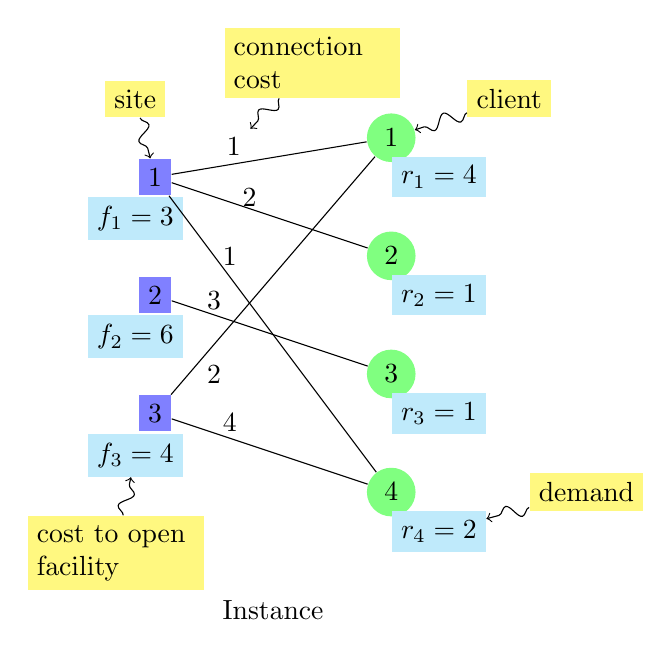
\begin{tikzpicture}[scale=0.5,decoration=snake]
    \node[fill=blue!50] (fac3) at (0,2) {$3$};
    \node[fill=blue!50] (fac2) at (0,5) {$2$};
    \node[fill=blue!50] (fac1) at (0,8) {$1$};

    \node[below,fill=cyan!25] (faclabel3) at (-.5,1.5) {$f_3=4$};
    \node[below,fill=cyan!25] (faclabel2) at (-.5,4.5) {$f_2=6$};
    \node[below,fill=cyan!25] (faclabel1) at (-.5,7.5) {$f_1=3$};

    \node[circle,fill=green!50] (client4) at (6,0) {$4$};
    \node[circle,fill=green!50] (client3) at (6,3) {$3$};
    \node[circle,fill=green!50] (client2) at (6,6) {$2$};
    \node[circle,fill=green!50] (client1) at (6,9) {$1$};

    \node[right,fill=cyan!25] (demand4) at (6,-1) {$r_4=2$};
    \node[right,fill=cyan!25] (demand3) at (6,2) {$r_3=1$};
    \node[right,fill=cyan!25] (demand2) at (6,5) {$r_2=1$};
    \node[right,fill=cyan!25] (demand1) at (6,8) {$r_1=4$};

    \foreach \from/\to in {fac3/client4,fac3/client1,fac2/client3,fac1/client4,fac1/client2,fac1/client1}
    \draw (\from)--(\to);

    % edge weight
    \node[above] (ew11) at (2,8.3) {$1$};
    \node[above] (ew12) at (2.4,7) {$2$};
    \node[above] (ew14) at (1.9,5.5) {$1$};
    \node[above] (ew23) at (1.5,4.4) {$3$};
    \node[above] (ew33) at (1.5,2.5) {$2$};
    \node[above] (ew34) at (1.9,1.3) {$4$};

    \node (label1) at (3,-3) {Instance};

    \pause
    % annotations
    \node[above,fill=yellow!50] (sites) at (-.5,9.5) {site}; 
    \draw[->,decorate] (sites) -- (fac1);
\pause
    \node[above,fill=yellow!50] (clients) at (9,9.5) {client};
    \draw[->,decorate] (clients) -- (client1);
\pause
    \node[right,fill=yellow!50] (demand) at (9.5,0) {demand};
    \draw[->,decorate] (demand) -- (demand4);
\pause
    \node[above,fill=yellow!50,text width=2cm] (fi) at (-1,-2.5) {cost to open facility};
    \draw[->,decorate] (fi) -- (faclabel3);
\pause
    \node[above,fill=yellow!50,text width=2cm] (edge) at (4,10) {connection cost};
    \draw[->,decorate] (edge) -- (ew11);
\pause
  \end{tikzpicture}
  \end{center}
\end{frame}

\begin{frame}
  \frametitle{Fault-tolerant Facility Placement Problem (FTFP)}

  \begin{center}
  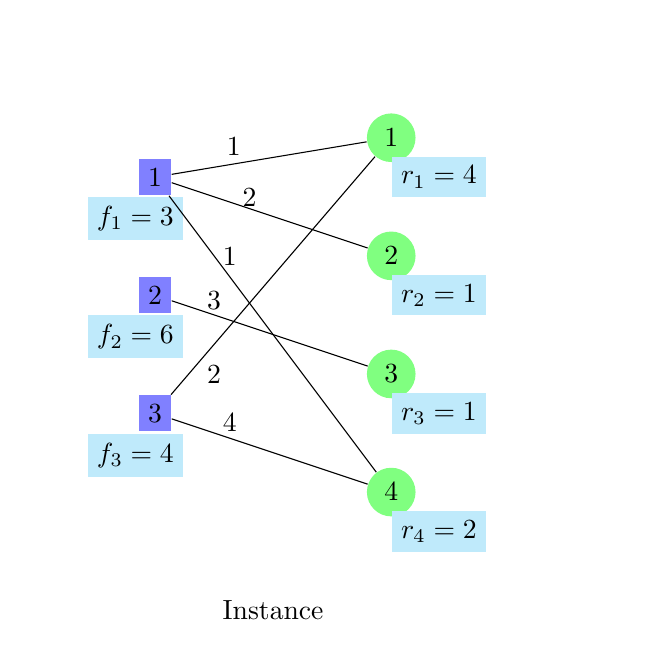
\begin{tikzpicture}[scale=0.5,decoration=snake]
    \node[fill=blue!50] (fac3) at (0,2) {$3$};
    \node[fill=blue!50] (fac2) at (0,5) {$2$};
    \node[fill=blue!50] (fac1) at (0,8) {$1$};

    \node[below,fill=cyan!25] (faclabel3) at (-.5,1.5) {$f_3=4$};
    \node[below,fill=cyan!25] (faclabel2) at (-.5,4.5) {$f_2=6$};
    \node[below,fill=cyan!25] (faclabel1) at (-.5,7.5) {$f_1=3$};

    \node[circle,fill=green!50] (client4) at (6,0) {$4$};
    \node[circle,fill=green!50] (client3) at (6,3) {$3$};
    \node[circle,fill=green!50] (client2) at (6,6) {$2$};
    \node[circle,fill=green!50] (client1) at (6,9) {$1$};

    \node[right,fill=cyan!25] (demand4) at (6,-1) {$r_4=2$};
    \node[right,fill=cyan!25] (demand3) at (6,2) {$r_3=1$};
    \node[right,fill=cyan!25] (demand2) at (6,5) {$r_2=1$};
    \node[right,fill=cyan!25] (demand1) at (6,8) {$r_1=4$};
    
    \foreach \from/\to in {fac3/client4,fac3/client1,fac2/client3,fac1/client4,fac1/client2,fac1/client1}
    \draw (\from)--(\to);

    % edge weight
    \node[above] (ew11) at (2,8.3) {$1$};
    \node[above] (ew12) at (2.4,7) {$2$};
    \node[above] (ew14) at (1.9,5.5) {$1$};
    \node[above] (ew23) at (1.5,4.4) {$3$};
    \node[above] (ew33) at (1.5,2.5) {$2$};
    \node[above] (ew34) at (1.9,1.3) {$4$};

    \node (label1) at (3,-3) {Instance};


    % remove annotations, use white, ugly solution
    \node[above,fill=white,color=white] (sites) at (-.5,9.5) {site}; 
    \draw[->,decorate,draw=none] (sites) -- (fac1);

    \node[above,fill=white,color=white] (clients) at (9,9.5) {client};
    \draw[->,decorate,draw=none] (clients) -- (client1);

    \node[right,fill=white,color=white] (demand) at (9.5,0) {demand};
    \draw[->,decorate,draw=none] (demand) -- (demand4);

    \node[above,fill=white,color=white,text width=2cm] (fi) at (-1,-2.5) {cost to open facility};
    \draw[->,decorate,draw=none] (fi) -- (faclabel3);

    \node[above,fill=white,color=white,text width=2cm] (edge) at (4,10) {connection cost};
    \draw[->,decorate,draw=none] (edge) -- (ew11);

  \end{tikzpicture}
  \end{center}
\end{frame}

%%% A feasible solution
\begin{frame}
  \frametitle{Feasible Integral Solution}
  \begin{figure}
    \centering
    \subfigure{
      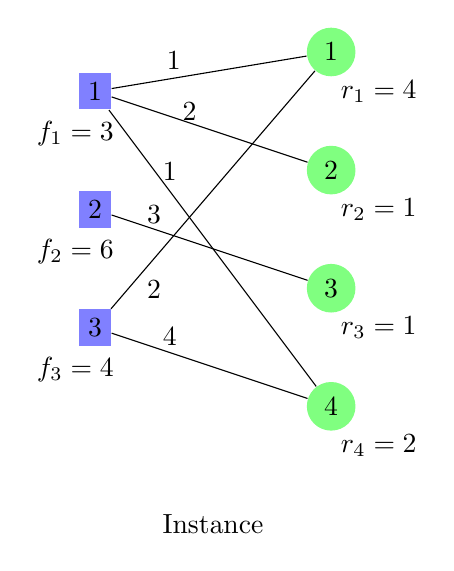
\begin{tikzpicture}[scale=0.5]
    \node[fill=blue!50] (fac3) at (0,2) {$3$};
    \node[fill=blue!50] (fac2) at (0,5) {$2$};
    \node[fill=blue!50] (fac1) at (0,8) {$1$};

    \node[below] (faclabel3) at (-.5,1.5) {$f_3=4$};
    \node[below] (faclabel2) at (-.5,4.5) {$f_2=6$};
    \node[below] (faclabel1) at (-.5,7.5) {$f_1=3$};

    \node[circle,fill=green!50] (client4) at (6,0) {$4$};
    \node[circle,fill=green!50] (client3) at (6,3) {$3$};
    \node[circle,fill=green!50] (client2) at (6,6) {$2$};
    \node[circle,fill=green!50] (client1) at (6,9) {$1$};

    \node[right] (demand4) at (6,-1) {$r_4=2$};
    \node[right] (demand3) at (6,2) {$r_3=1$};
    \node[right] (demand2) at (6,5) {$r_2=1$};
    \node[right] (demand1) at (6,8) {$r_1=4$};
    
    \foreach \from/\to in {fac3/client4,fac3/client1,fac2/client3,fac1/client4,fac1/client2,fac1/client1}
    \draw (\from)--(\to);

    % edge weight
    \node[above] (ew11) at (2,8.3) {$1$};
    \node[above] (ew12) at (2.4,7) {$2$};
    \node[above] (ew14) at (1.9,5.5) {$1$};
    \node[above] (ew23) at (1.5,4.4) {$3$};
    \node[above] (ew33) at (1.5,2.5) {$2$};
    \node[above] (ew34) at (1.9,1.3) {$4$};

    \node (label1) at (3,-3) {Instance};
  \end{tikzpicture}
}
  \hspace{.25in}
  \subfigure{
    \centering
    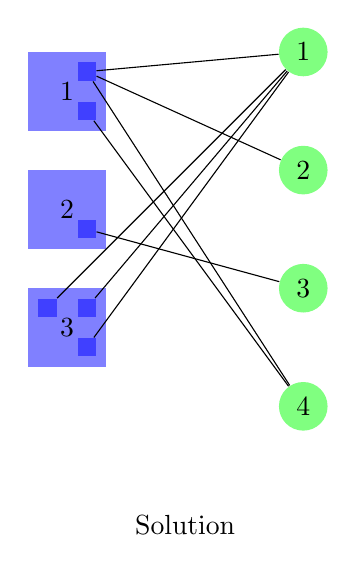
\begin{tikzpicture}[scale=0.5]
    \node[fill=blue!50,minimum size=1cm] (fac3) at (0,2) {$3$};
    \node[fill=blue!75,minimum size=.2cm] (fac33) at (.5,1.5) {};
    \node[fill=blue!75,minimum size=.2cm] (fac32) at (.5,2.5) {};
    \node[fill=blue!75,minimum size=.2cm] (fac31) at (-.5,2.5) {};

    \node[fill=blue!50,minimum size=1cm] (fac2) at (0,5) {$2$};
    \node[fill=blue!75,minimum size=.2cm] (fac21) at (.5,4.5) {};

    \node[fill=blue!50,minimum size=1cm] (fac1) at (0,8) {$1$};
    \node[fill=blue!75,minimum size=.2cm] (fac12) at (.5,7.5) {};
   \node[fill=blue!75,minimum size=.2cm] (fac11) at (.5,8.5) {};

    \node[circle,fill=green!50] (client4) at (6,0) {$4$};
    \node[circle,fill=green!50] (client3) at (6,3) {$3$};
    \node[circle,fill=green!50] (client2) at (6,6) {$2$};
    \node[circle,fill=green!50] (client1) at (6,9) {$1$};
    
    \foreach \from/\to in {fac31/client1,fac32/client1,fac33/client1,fac11/client1,fac11/client2,fac11/client4,fac21/client3,fac12/client4}
        \draw (\from)--(\to);
    
    \node (label1) at (3,-3) {Solution};
  \end{tikzpicture}
}
\end{figure}

  Cost is $2f_1 + f_2 + 3f_3 + d_{11} + d_{12} + 2d_{14} +
  d_{23} + 3d_{31} = 38$
\end{frame}

\begin{frame}
  \frametitle{Optimal Integral Solution}
  
  \begin{figure}
    \centering
    \subfigure{
  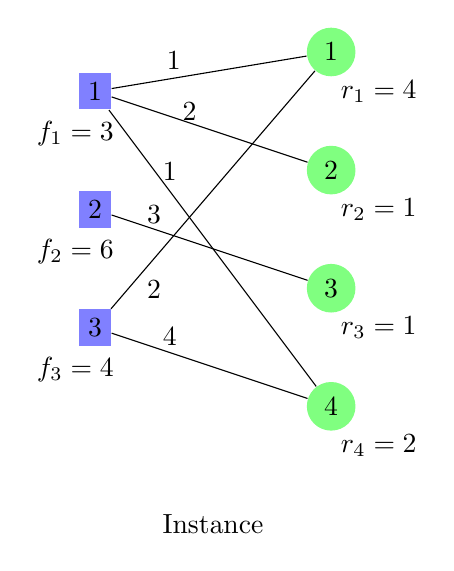
\begin{tikzpicture}[scale=0.5]
    \node[fill=blue!50] (fac3) at (0,2) {$3$};
    \node[fill=blue!50] (fac2) at (0,5) {$2$};
    \node[fill=blue!50] (fac1) at (0,8) {$1$};

    \node[below] (faclabel3) at (-.5,1.5) {$f_3=4$};
    \node[below] (faclabel2) at (-.5,4.5) {$f_2=6$};
    \node[below] (faclabel1) at (-.5,7.5) {$f_1=3$};

    \node[circle,fill=green!50] (client4) at (6,0) {$4$};
    \node[circle,fill=green!50] (client3) at (6,3) {$3$};
    \node[circle,fill=green!50] (client2) at (6,6) {$2$};
    \node[circle,fill=green!50] (client1) at (6,9) {$1$};

    \node[right] (demand4) at (6,-1) {$r_4=2$};
    \node[right] (demand3) at (6,2) {$r_3=1$};
    \node[right] (demand2) at (6,5) {$r_2=1$};
    \node[right] (demand1) at (6,8) {$r_1=4$};
    
    \foreach \from/\to in {fac3/client4,fac3/client1,fac2/client3,fac1/client4,fac1/client2,fac1/client1}
    \draw (\from)--(\to);

    % edge weight
    \node[above] (ew11) at (2,8.3) {$1$};
    \node[above] (ew12) at (2.4,7) {$2$};
    \node[above] (ew14) at (1.9,5.5) {$1$};
    \node[above] (ew23) at (1.5,4.4) {$3$};
    \node[above] (ew33) at (1.5,2.5) {$2$};
    \node[above] (ew34) at (1.9,1.3) {$4$};

    \node (label1) at (3,-3) {Instance};
  \end{tikzpicture}
}    
  \hspace{.25in}
\subfigure{
    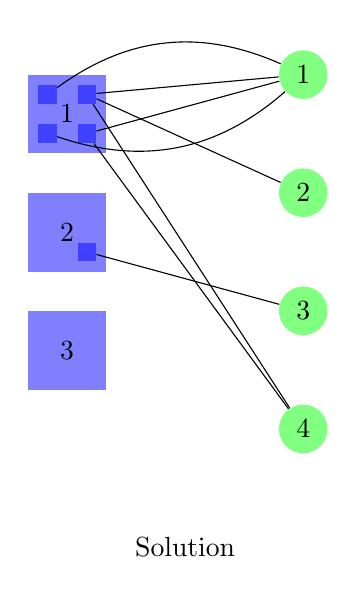
\begin{tikzpicture}[scale=0.5]
    \node[fill=blue!50,minimum size=1cm] (fac3) at (0,2) {$3$};

    \node[fill=blue!50,minimum size=1cm] (fac2) at (0,5) {$2$};
    \node[fill=blue!75,minimum size=.2cm] (fac21) at (.5,4.5) {};

    \node[fill=blue!50,minimum size=1cm] (fac1) at (0,8) {$1$};
    \node[fill=blue!75,minimum size=.2cm] (fac14) at (-.5,7.5) {};
    \node[fill=blue!75,minimum size=.2cm] (fac13) at (-.5,8.5) {};
    \node[fill=blue!75,minimum size=.2cm] (fac12) at (.5,7.5) {};
    \node[fill=blue!75,minimum size=.2cm] (fac11) at (.5,8.5) {};

    \node[circle,fill=green!50] (client4) at (6,0) {$4$};
    \node[circle,fill=green!50] (client3) at (6,3) {$3$};
    \node[circle,fill=green!50] (client2) at (6,6) {$2$};
    \node[circle,fill=green!50] (client1) at (6,9) {$1$};
    
    \foreach \from/\to in {fac11/client1,fac12/client1,fac11/client2,fac11/client4,fac12/client4,fac21/client3}
        \draw (\from)--(\to);

    \draw[bend left] (fac13) to node (ew13) {} (client1);
    \draw[bend right] (fac14) to node (ew14) {} (client1);
    \node (label1) at (3,-3) {Solution};
  \end{tikzpicture}
  }
  \end{figure}

  Cost is $4f_1 + 1f_2 + 0f_3 + 4d_{11} + d_{12} + 2d_{14} +
  d_{23} = 29$
\end{frame}

%% 2. Results: 1.575 rounding, hard example on dual-fitting

%% 3. Techniques:
%% 3.1 Demand Reduction: why, what (end product) and how (take floor)
%%     implication: reduction to FTFL, 1 + O(m/Q) approximation
%% 3.2 Adaptive Partitioning: why, what and how
%%     why: to use UFL-like rounding
%%     what: facility points and unit demand points, \barx and \bary with mu and nu
%%           properties...
%%     how: unit chunk, best client, primary, non-primary, overlap of neighborhood
%%
%% 3.3 Rounding: fault-tolerant made easy, all ratios preserved
%%     the 1.575 rounding is subtle
%% 3.4 Greedy, Dual-fitting, and hard example for local-charging

%% 4. Open problems and future work
%%     - dual-fitting for FTFP
%%     - 1.463 for UFL
\end{document}
